        \documentclass{standalone}
        \usepackage{tikz}
        \begin{document}
        \fontsize{16px}{16px}\selectfont
        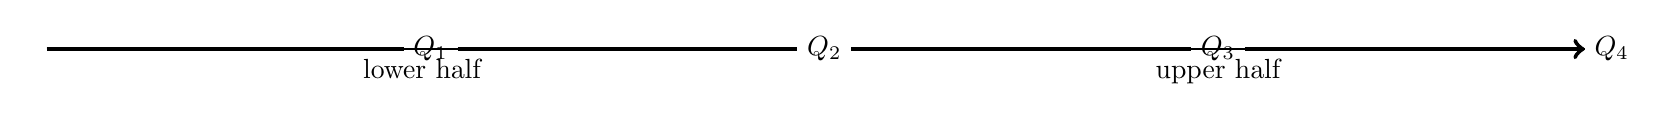
\begin{tikzpicture}


    \node at (0,0) (nodeA) {};
    \node at (5,0) (nodeB) {$Q_1$};
    \node at (10,0) (nodeC) {$Q_2$};
    \node at (15,0) (nodeD) {$Q_3$};
    \node at (20,0) (nodeE) {$Q_4$};
    \draw[ultra thick](nodeA) -- (nodeB);
    \draw[ultra thick](nodeB) -- (nodeC);
    \draw(nodeA) -- (nodeC) node [midway, below] (TextNode) {lower half};
    \draw[ultra thick](nodeC) -- (nodeD);
    \draw[ultra thick,arrows=->](nodeD) -- (nodeE);
    \draw (nodeC) -- (nodeE) node [midway, below] (TextNode) {upper half};
        \end{tikzpicture}
        \end{document}
